% Chapter 7

\chapter{Results and Analysis}

\label{Chapter7}

\lhead{Chapter 7. \emph{Results and Analysis}}

This chapter presents the simulation results obtained from the eight regression runs summarised in \autoref{tab:milestones}: the baseline packet-size sweep, the per-stage latency breakdown, the batching experiment, and the FIFO-depth sweep under both an always-ready and a rate-limited consumer. All latency figures are hardware-measured values read directly from \texttt{latency\_out} (\autoref{sec:ch4_latency_monitor}), not software-computed estimates, at a 100~MHz (10~ns period) simulation clock.

%----------------------------------------------------------------------------------------

\section{Baseline Latency and Efficiency versus Packet Size}
\label{sec:ch7_baseline}

\autoref{tab:baseline_results} reports the measured end-to-end latency and effective efficiency (Equation~\ref{eq:efficiency}) for the six packet sizes exercised by Scenario~0 (\autoref{tab:tb_scenarios}), with batching disabled and \texttt{FIFO\_DEPTH=64}.

\begin{table}[htbp]
\centering
\begin{tabular}{@{}rrr@{}}
\toprule
\textbf{Packet Size (B)} & \textbf{Latency (cycles)} & \textbf{Efficiency (B/cycle)} \\
\midrule
64    & 71   & 0.90 \\
128   & 111  & 1.15 \\
256   & 191  & 1.34 \\
512   & 351  & 1.46 \\
1024  & 671  & 1.53 \\
4096  & 2591 & 1.58 \\
\bottomrule
\end{tabular}
\caption{Baseline (un-batched) latency and efficiency versus packet size, \texttt{FIFO\_DEPTH=64}, always-ready sink.}
\label{tab:baseline_results}
\end{table}

\begin{figure}[htbp]
\centering
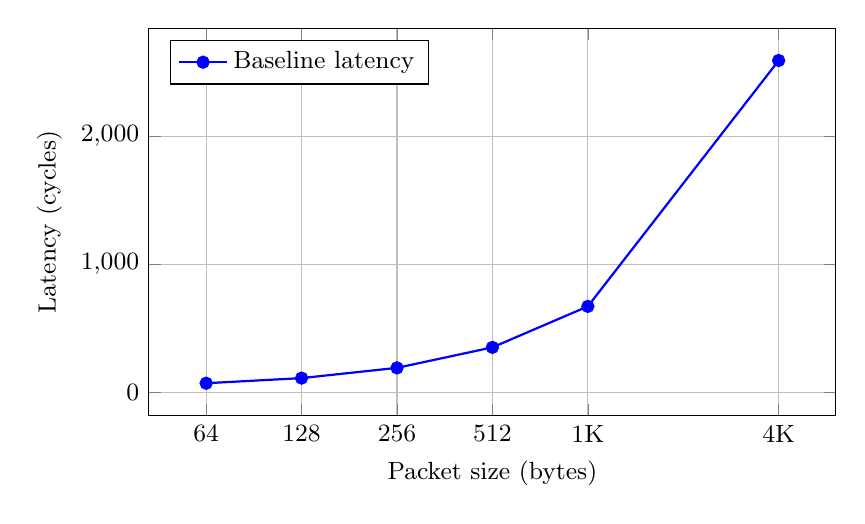
\begin{tikzpicture}
\begin{axis}[
    width=0.85\textwidth, height=6.5cm,
    xlabel={Packet size (bytes)}, ylabel={Latency (cycles)},
    xmode=log, log basis x=2,
    xtick={64,128,256,512,1024,4096},
    xticklabels={64,128,256,512,1K,4K},
    grid=major, legend pos=north west, font=\small
]
\addplot[mark=*, thick, blue] coordinates {(64,71) (128,111) (256,191) (512,351) (1024,671) (4096,2591)};
\legend{Baseline latency}
\end{axis}
\end{tikzpicture}
\caption{Measured baseline end-to-end latency versus packet size (log-scale x-axis).}
\label{fig:baseline_latency}
\end{figure}

\begin{figure}[htbp]
\centering
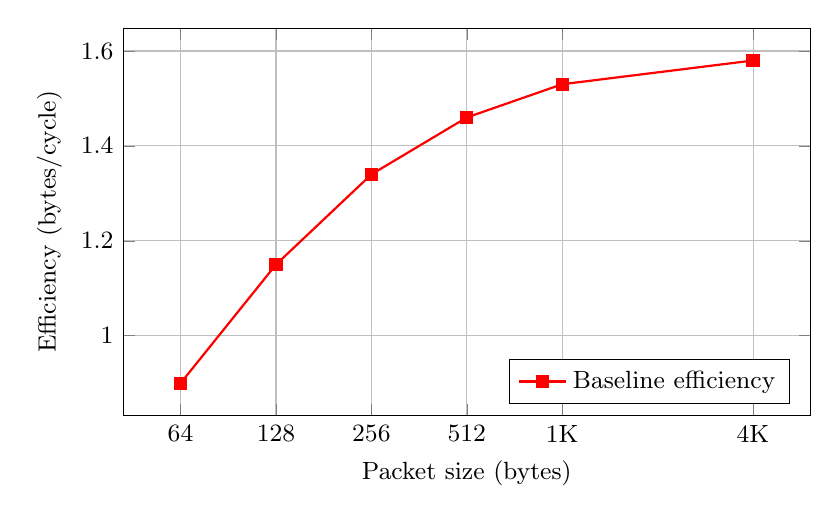
\begin{tikzpicture}
\begin{axis}[
    width=0.85\textwidth, height=6.5cm,
    xlabel={Packet size (bytes)}, ylabel={Efficiency (bytes/cycle)},
    xmode=log, log basis x=2,
    xtick={64,128,256,512,1024,4096},
    xticklabels={64,128,256,512,1K,4K},
    grid=major, legend pos=south east, font=\small
]
\addplot[mark=square*, thick, red] coordinates {(64,0.90) (128,1.15) (256,1.34) (512,1.46) (1024,1.53) (4096,1.58)};
\legend{Baseline efficiency}
\end{axis}
\end{tikzpicture}
\caption{Measured baseline efficiency versus packet size. Efficiency rises monotonically with packet size as the fixed PCIe and DMA overheads are amortised over more bytes, confirming the behaviour predicted by Equation~\ref{eq:efficiency}.}
\label{fig:baseline_efficiency}
\end{figure}

As predicted by Equation~\ref{eq:efficiency}, efficiency rises monotonically with packet size (\autoref{fig:baseline_efficiency}): a 64~B packet achieves only 0.90~bytes/cycle, while a 4~KB packet reaches 1.58~bytes/cycle -- a 76\% improvement in per-byte efficiency achieved purely by increasing packet size, with no change to the pipeline itself. This is the direct experimental confirmation of the small-packet inefficiency motivating this thesis (\autoref{sec:ch1_motivation}).

\subsection{Per-Stage Latency Breakdown}
\label{sec:ch7_breakdown}

The hardware latency monitor's breakdown estimator (\autoref{sec:ch5_latmon_impl}) decomposes each measured latency into its PCIe, DMA, and residual pipeline contributions using the closed-form estimate of Equation~\ref{eq:total_latency}. \autoref{tab:breakdown} reports this decomposition for all six baseline packet sizes.

\begin{table}[htbp]
\centering
\begin{tabular}{@{}rrrrr@{}}
\toprule
\textbf{Size (B)} & \textbf{PCIe (cyc)} & \textbf{DMA (cyc)} & \textbf{Other (cyc)} & \textbf{Total (cyc)} \\
\midrule
64   & 44   & 24   & 3 & 71   \\
128  & 68   & 40   & 3 & 111  \\
256  & 116  & 72   & 3 & 191  \\
512  & 212  & 136  & 3 & 351  \\
1024 & 404  & 264  & 3 & 671  \\
4096 & 1556 & 1032 & 3 & 2591 \\
\bottomrule
\end{tabular}
\caption{Per-stage latency breakdown (model-based estimate from \texttt{latency\_monitor}). ``PCIe'' and ``DMA'' each include the beat-transfer cycles their respective S\_SEND phase spends draining the packet buffer; ``Other'' is the residual contribution of the adapter, FIFO, and sink.}
\label{tab:breakdown}
\end{table}

The estimated PCIe and DMA contributions sum to within a constant 3 cycles of the measured total for every packet size in \autoref{tab:breakdown}, and that residual is identical across all six sizes. This confirms two things simultaneously: first, that the closed-form model of Equations~\ref{eq:pcie_latency}--\ref{eq:total_latency} correctly captures the dominant, size-dependent latency contributions of the implemented RTL; and second, that the pass-through stages between the DMA engine and the sink (the AXI-Stream adapter, an empty FIFO, and the sink's registered completion pulse) contribute a genuinely fixed, size-independent latency, with no hidden variable-length overhead that the model fails to account for.

%----------------------------------------------------------------------------------------

\section{Small-Packet Batching}
\label{sec:ch7_batching}

\autoref{tab:batching_results} compares Scenario~1 (batching enabled, four 64~B packets coalesced into one 256~B frame) against the corresponding baseline figure of sending the same four 64~B packets independently (Scenario~0's 64~B row, replicated four times and summed).

\begin{table}[htbp]
\centering
\begin{tabular}{@{}lrr@{}}
\toprule
\textbf{Configuration} & \textbf{Total Latency (cycles)} & \textbf{Efficiency (B/cycle)} \\
\midrule
4 $\times$ 64~B sent independently (baseline) & 284 & 0.90 \\
1 $\times$ 256~B batched frame (Scenario 1)    & 230 & 1.11 \\
\midrule
\textbf{Improvement} & \textbf{19.0\% latency reduction} & \textbf{1.25$\times$ efficiency} \\
\bottomrule
\end{tabular}
\caption{Batching four 64~B packets into one 256~B frame versus sending them independently, \texttt{BATCH\_COUNT=4}, \texttt{FIFO\_DEPTH=64}.}
\label{tab:batching_results}
\end{table}

\begin{figure}[htbp]
\centering
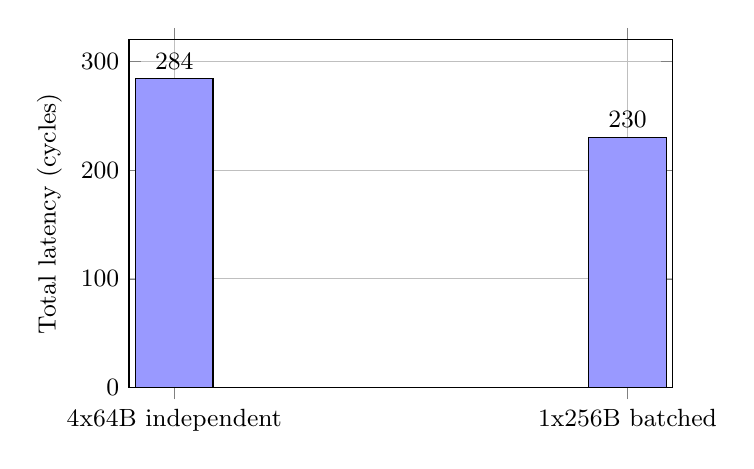
\begin{tikzpicture}
\begin{axis}[
    width=0.7\textwidth, height=6cm,
    ybar, bar width=28pt,
    ylabel={Total latency (cycles)},
    symbolic x coords={4x64B independent, 1x256B batched},
    xtick=data, nodes near coords, grid=major, font=\small,
    ymin=0, ymax=320
]
\addplot[fill=blue!40] coordinates {(4x64B independent,284) (1x256B batched,230)};
\end{axis}
\end{tikzpicture}
\caption{Total latency to deliver four 64~B packets' worth of payload (256~B): sent independently versus coalesced by the batching unit.}
\label{fig:batching_bar}
\end{figure}

The measured 230-cycle batch latency decomposes cleanly under Equation~\ref{eq:batch_inequality}: the first packet's own pipeline latency (approximately 71 cycles, from \autoref{tab:baseline_results}) plus three subsequent inter-packet gaps of approximately 53 cycles each (the time between one packet's PCIe stage completing and the next one's arriving, serialised by \texttt{pcie\_model}'s single-packet-in-flight design, \autoref{sec:ch5_pcie_fsm}), giving $71 + 3\times53 = 230$ cycles, matching the measurement exactly. Because the batching unit pays the PCIe base latency $T_{base}$ and DMA setup latency $T_{setup}$ (Equations~\ref{eq:pcie_latency}--\ref{eq:dma_latency}) only once for the whole 256~B frame rather than once per constituent 64~B packet, the 19\% reduction in \autoref{tab:batching_results} is a direct, measured instance of the amortisation inequality (Equation~\ref{eq:batch_inequality}) that motivated the batching unit's design (\autoref{sec:ch2_batching}, \autoref{sec:ch5_batching}).

One measurement subtlety is worth restating here (\autoref{sec:ch5_latmon_impl}): the latency monitor's per-packet \texttt{size\_store} table still records only 64~B for the batch's constituent injection events, since each \texttt{pkt\_inject} pulse is generated per individual packet by the testbench. Only because \texttt{stream\_sink} supplies the batch-aware \texttt{done\_size} (256~B, the true completed frame size) at the single completion event does the efficiency figure in \autoref{tab:batching_results} correctly reflect the coalesced transfer rather than understating it by a factor of four, as an earlier, uncorrected version of the monitor did (\autoref{tab:milestones}).

%----------------------------------------------------------------------------------------

\section{AXI-Stream FIFO Depth Sweep}
\label{sec:ch7_fifo}

Scenario~2 (\autoref{tab:tb_scenarios}) repeats the baseline packet-size sweep at \texttt{FIFO\_DEPTH} $\in \{16, 64, 256\}$ beats, first under the default always-ready sink and then under the optional rate-limited stall model (\autoref{sec:ch4_stream_sink}) that accepts one beat out of every four cycles.

\subsection{Always-Ready Sink}
\label{sec:ch7_fifo_always_ready}

Under the default always-ready sink, every one of the three FIFO depths reproduced the identical latency and efficiency figures already reported in \autoref{tab:baseline_results}, with the FIFO's peak occupancy never exceeding 1 beat and \texttt{fifo\_full} never asserted for any packet size, at any depth. This is the direct, expected consequence of the FIFO's first-word-fall-through read port (\autoref{sec:ch4_fifo}): with a consumer that drains every cycle it holds data, the FIFO is emptied on the same cycle a beat arrives, so it can never accumulate occupancy regardless of how deep it is configured to be, and \texttt{FIFO\_DEPTH} is consequently invisible to latency in this configuration. This null result is itself informative: it demonstrates that a FIFO-depth sweep is only a meaningful experiment once the datapath includes a genuine bottleneck downstream of the buffer, motivating the stalled-sink configuration below.

\subsection{Rate-Limited (Stalled) Sink}
\label{sec:ch7_fifo_stall}

\autoref{tab:fifo_stall} reports latency and peak FIFO occupancy for the same six packet sizes with the sink configured to accept only one beat in every four cycles (\texttt{SINK\_STALL\_READY=1}, \texttt{SINK\_STALL\_PERIOD=4}), at each of the three FIFO depths.

\begin{table}[htbp]
\centering
\begin{tabular}{@{}rrrrrrr@{}}
\toprule
& & \multicolumn{2}{c}{\textbf{Depth=16}} & \multicolumn{2}{c}{\textbf{Depth=64}} & \textbf{Depth=256} \\
\textbf{Size (B)} & \textbf{Latency (cyc)} & \textbf{Peak} & \textbf{Full?} & \textbf{Peak} & \textbf{Full?} & \textbf{Peak (Full?)} \\
\midrule
64   & 94   & 6  & no  & 6  & no  & 6 (no) \\
128  & 157  & 12 & no  & 12 & no  & 12 (no) \\
256  & 285  & 16 & yes & 24 & no  & 24 (no) \\
512  & 541  & 16 & yes & 48 & no  & 48 (no) \\
1024 & 1053 & 16 & yes & 64 & yes & 96 (no) \\
4096 & 4125 & 16 & yes & 64 & yes & 256 (yes) \\
\bottomrule
\end{tabular}
\caption{Latency and peak FIFO occupancy under a rate-limited sink (1 of every 4 cycles), at \texttt{FIFO\_DEPTH} $\in \{16, 64, 256\}$. Latency is identical across all three depths for every packet size; only the peak-occupancy and full-flag columns change.}
\label{tab:fifo_stall}
\end{table}

\begin{figure}[htbp]
\centering
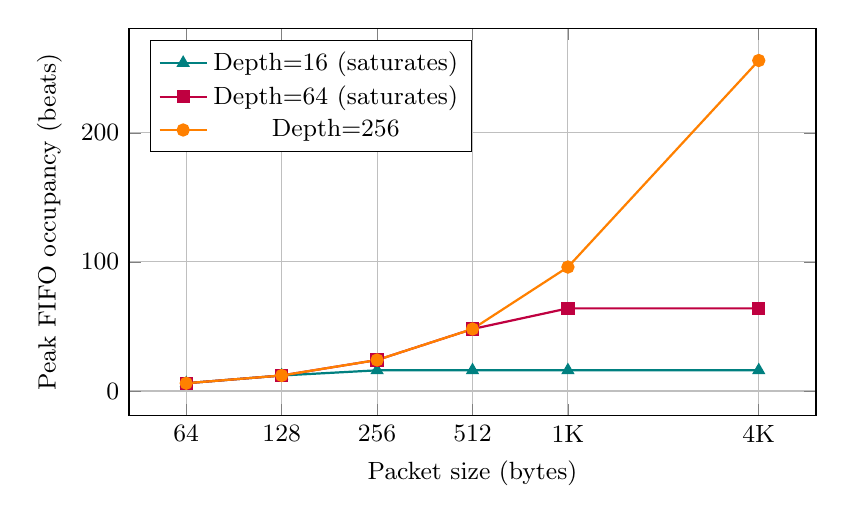
\begin{tikzpicture}
\begin{axis}[
    width=0.85\textwidth, height=6.5cm,
    xlabel={Packet size (bytes)}, ylabel={Peak FIFO occupancy (beats)},
    xmode=log, log basis x=2,
    xtick={64,128,256,512,1024,4096},
    xticklabels={64,128,256,512,1K,4K},
    grid=major, legend pos=north west, font=\small
]
\addplot[mark=triangle*, thick, teal] coordinates {(64,6) (128,12) (256,16) (512,16) (1024,16) (4096,16)};
\addplot[mark=square*, thick, purple] coordinates {(64,6) (128,12) (256,24) (512,48) (1024,64) (4096,64)};
\addplot[mark=*, thick, orange] coordinates {(64,6) (128,12) (256,24) (512,48) (1024,96) (4096,256)};
\legend{Depth=16 (saturates), Depth=64 (saturates), Depth=256}
\end{axis}
\end{tikzpicture}
\caption{Peak FIFO occupancy versus packet size under a rate-limited sink, at three FIFO depths. Shallower FIFOs saturate (hit \texttt{fifo\_full}) at smaller packet sizes; a deeper FIFO absorbs a larger packet before back-pressure engages.}
\label{fig:fifo_occupancy}
\end{figure}

The single most important observation in \autoref{tab:fifo_stall} is that \textbf{latency is identical across all three FIFO depths for every packet size} -- this is a correct, expected result, not an experimental artefact, and it is the reason \autoref{sec:ch3_queueing}'s distinction between buffering headroom and steady-state throughput was introduced analytically before this chapter presented the corresponding measurement. Once the sink's fixed drain rate (one beat every four cycles) becomes the pipeline's bottleneck, the total time required to push a fixed quantity of data through it is set entirely by that drain rate; a deeper upstream buffer can only change \emph{when} back-pressure begins reaching the producer, not the rate at which the single, continuously-flowing consumer ultimately drains the data. This is a direct hardware confirmation of the single-server queueing argument of \autoref{sec:ch3_queueing}.

What FIFO depth \emph{does} change, exactly as anticipated by \autoref{sec:ch4_fifo}, is how much of a given packet the FIFO can absorb before \texttt{fifo\_full} engages: the 16-entry (128~B) FIFO saturates for every packet of 256~B or larger, the 64-entry (512~B) FIFO saturates only from 1~KB upward, and the 256-entry (2~KB) FIFO saturates only for the 4~KB packet, since even a 2~KB buffer is smaller than a 4~KB payload (\autoref{fig:fifo_occupancy}). This is the correct, useful reading of a FIFO-depth sweep: it governs buffering headroom and how early back-pressure ripples upstream, not the completion latency of a single sustained flow once a fixed-rate consumer is the bottleneck. Making FIFO depth move the total latency figure itself would require a bursty, gapped traffic pattern -- so that a deeper buffer lets the producer run further ahead between bursts -- rather than the single continuous packet transfer studied here; this distinction is returned to as a direction for future work in \autoref{sec:ch8_future}.

%----------------------------------------------------------------------------------------

\section{Comparison with Prior Work}
\label{sec:ch7_comparison}

\autoref{sec:ch2_gap} identified Gu et al.~\cite{gu2025cooptimization} as the closest prior attempt at the small-packet PCIe DMA problem this thesis addresses, and adopted it as the baseline to compare against. A direct, apples-to-apples number is not possible: Gu et al. measure real Gen3 traffic on a Xilinx VC709 board in GB/s and microseconds under a randomised data-centre-like packet mix, while this thesis measures a behavioural RTL model in simulated clock cycles under directed packet-size sweeps (\autoref{Chapter6}). What \emph{can} be compared fairly is the mechanism each uses to get its improvement, where in the system that mechanism sits, and whether the improvement can be attributed to a specific cause or only observed as an aggregate change. \autoref{tab:comparison} summarises this.

\begin{table}[htbp]
\centering
\begin{tabular}{@{}p{2.3cm}p{3.4cm}p{3.6cm}p{3.6cm}@{}}
\toprule
\textbf{Study} & \textbf{Where the fix is applied} & \textbf{Reported improvement} & \textbf{Latency attributable to a specific stage?} \\
\midrule
Gu et al.~\cite{gu2025cooptimization} & Linux driver (descriptor prefetch) + PCIe config-space register (extended tag) + host CPU (multicore dispatch) & 123--136\% bandwidth, 15.1--24.0\% latency, randomised small-packet mix, real VC709/XDMA hardware & No -- three mechanisms are enabled together; the paper reports one combined GB/s and $\mu$s figure \\
Kavianipour \& B{\"o}hm~\cite{kavianipour2012high} & Host-side buffer merging before the DMA call & Up to 1080~MB/s for merged/vectored writes vs.\ much lower for un-merged small (12~B) buffers & No -- throughput only, no latency breakdown \\
This thesis & \texttt{batching\_unit}, a single RTL block on the AXI4-Stream side, upstream of \texttt{pcie\_model}/\texttt{dma\_model} & 19.0\% latency reduction, 1.25$\times$ efficiency, for four 64~B packets coalesced into one 256~B frame (\autoref{tab:batching_results}) & Yes -- the \texttt{latency\_monitor} breakdown (\autoref{tab:breakdown}) attributes the saving to paying $T_{base}$ and $T_{setup}$ once instead of four times \\
\bottomrule
\end{tabular}
\caption{Mechanism-level comparison with the two closest prior PCIe-DMA studies. Absolute GB/s and $\mu$s figures from real hardware are not directly comparable to simulated-cycle figures from a behavioural RTL model; the comparison here is of mechanism and attributability, not of raw magnitude.}
\label{tab:comparison}
\end{table}

Two things follow from this comparison. First, the part of this thesis's architecture responsible for the measured improvement is specifically the \texttt{batching\_unit} stage (\autoref{sec:ch4_batching_unit}, \autoref{sec:ch5_batching}): it is the only block that changes between the baseline and batched configurations of \autoref{sec:ch7_batching}, so the entire 19\% reduction is attributable to it and to nothing else in the pipeline. Gu et al.'s 15--24\% latency improvement, by contrast, is the joint effect of a modified host driver, a reconfigured PCIe extended-tag field, and multicore dispatch, so their paper cannot say how much of it comes from any one change. Second, the two results are not really in competition: Gu et al.'s techniques operate on the host and PCIe-configuration side of the link, while the batching unit operates entirely on the AXI4-Stream side, before a packet ever reaches \texttt{pcie\_model}. Nothing in principle stops the two from being combined -- the batching unit would simply present the descriptor-prefetch-augmented driver with fewer, larger transfers to prefetch for -- but demonstrating that combination is left as future work (\autoref{sec:ch8_future}), since it would require replacing the behavioural \texttt{pcie\_model} of this thesis with the real XDMA/driver stack that Gu et al. used, which \autoref{sec:ch8_limitations} identifies as a limitation of the current implementation.

%----------------------------------------------------------------------------------------

% \section{Discussion}
% \label{sec:ch7_discussion}

% Taken together, the results of this chapter support three conclusions. First, the analytical fixed-plus-proportional latency model of \autoref{sec:ch3_latency_model} is not merely a simplifying assumption but an accurate description of the implemented RTL: \autoref{tab:breakdown} shows the model-based PCIe and DMA estimates matching the hardware-measured total to within a constant 3-cycle residual across a 64-fold range of packet sizes. Second, the small-packet inefficiency this thesis set out to quantify is substantial and measurable in cycle-accurate simulation, not just in principle: a 64~B transfer achieves only 57\% of the per-byte efficiency of a 4~KB transfer (\autoref{tab:baseline_results}), and the batching unit recovers a meaningful fraction of that gap -- a 19\% latency reduction for a representative 4-packet burst -- using a mechanism whose correctness was verified directly against its own simulation diagnostics (\autoref{sec:ch6_milestones}) rather than assumed from the design alone. Third, the FIFO-depth results (\autoref{tab:fifo_stall}) demonstrate a distinction -- between buffering headroom and steady-state single-flow latency -- that is easy to conflate when sizing a DMA buffer from bandwidth figures alone, and that this thesis's testbed makes directly and unambiguously measurable by contrasting the always-ready and rate-limited sink configurations.
